\newpage
\subsection{Caso d'uso UC11 - Registrazione API}
\label{UC11}
\begin{figure}[ht]
	\centering
	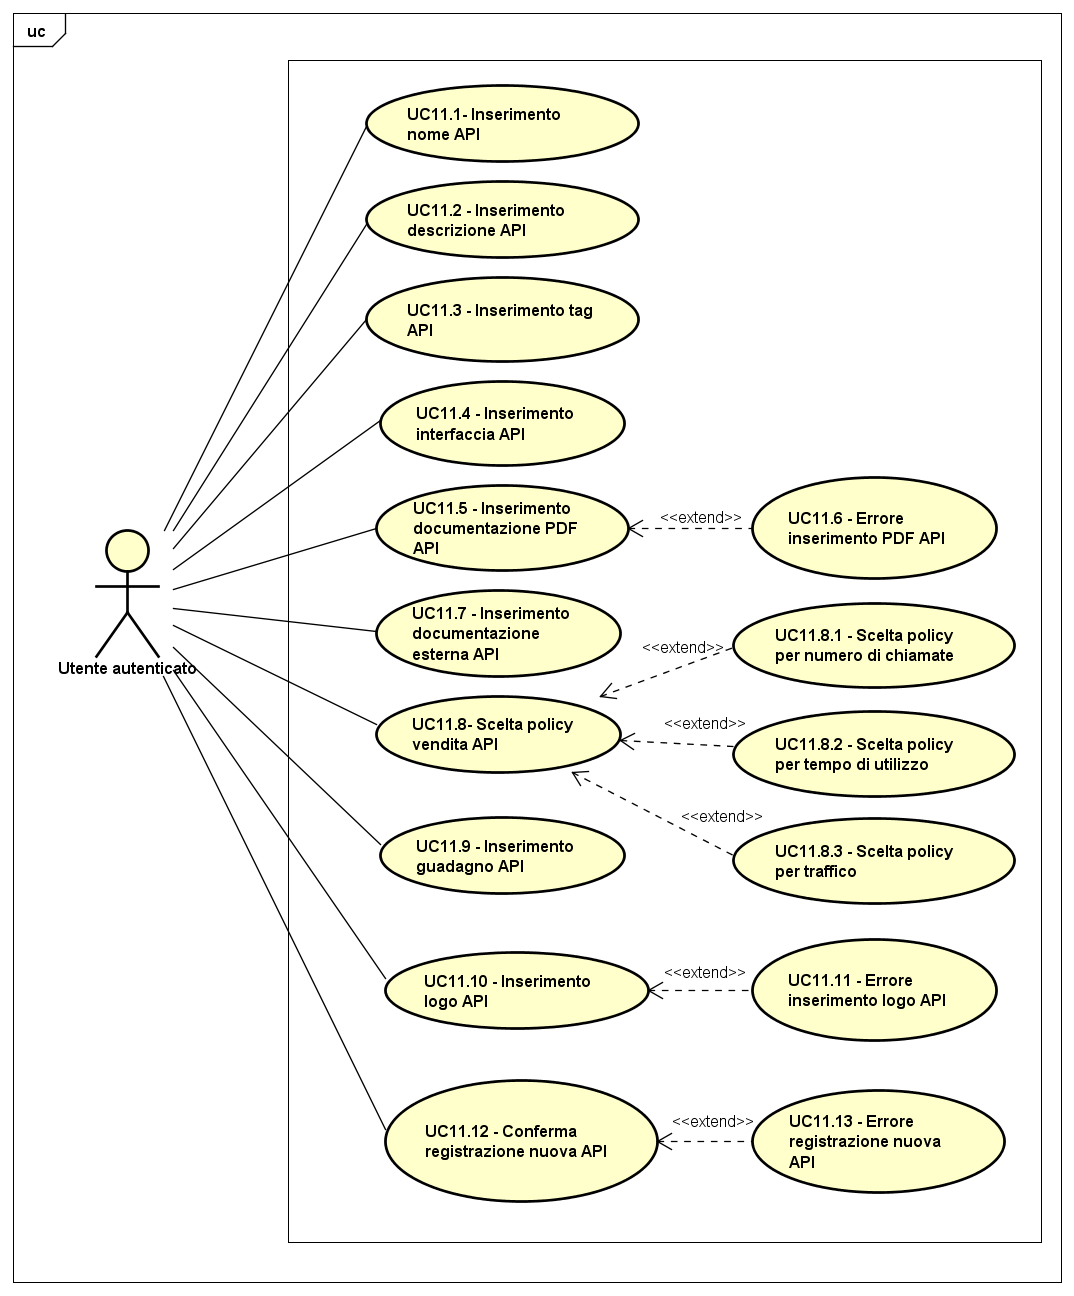
\includegraphics[scale=0.45]{UML/UC11.png}
	\caption{UC11: Registrazione API}
\end{figure}

\begin{longtable}{ l | p{11cm}}
	\hline
	\rowcolor{Gray}
	\multicolumn{2}{c}{UC11 - Registrazione API}\\
	\hline
	
	 \textbf{Attori} & Utente autenticato  \\
	\textbf{Descrizione} & L'attore può registrare la propria API sul marketplace \\
	\textbf{Pre-Condizioni} & L'attore ha visitato la pagina relativa alla registrazione di una nuova API \\
	\textbf{Post-Condizioni} & L'attore ha registrato la propria API sul marketplace \\
	\textbf{Scenario Principale} & 
	\begin{enumerate*}[label=(\arabic*.),itemjoin={\newline}]
		\item L'attore può inserire il nome dell'API (UC11.1)
		\item L'attore può inserire la descrizione dell'API (UC11.2)
		\item L'attore può inserire i tag dell'API (UC11.3)
		\item L'attore può inserire l'interfaccia pubblica dell'API (UC11.4)
		\item L'attore può inserire il link esterno alla documentazione (UC11.5)
		\item L'attore può inserire il file di documentazione caricato  (UC11.6)
		\item L'attore può inserire il prezzo base per l'API (UC11.7)
		\item L'attore può confermare i dati inseriti e continuare con l'operazione (UC11.8)
	\end{enumerate*}\\
	\textbf{Scenario Principale} & 
	\begin{enumerate*}[label=(\arabic*.),itemjoin={\newline}]
		\item L'attore riceve un avviso che l'operazione non è andata a buon fine per motivi legati ai dati inseriti (UC11.9)
	\end{enumerate*}\\
\end{longtable}

\paragraph{Caso d'uso UC11.1: Inserimento nome API}
\label{UC11_1}

\begin{minipage}{\linewidth}
	\begin{tabular}{ l | p{11cm}}
		\hline
		\rowcolor{Gray}
		\multicolumn{2}{c}{UC11.1 - Inserimento nome API} \\
		\hline
		\textbf{Attori} & Utente autenticato \\
		\textbf{Descrizione} & L'attore inserisce il nome relativo ad una propria API\\
		\textbf{Pre-Condizioni} & L'attore si trova nella schermata per la registrazione di un API\\
		\textbf{Post-Condizioni} & L'attore ha inserito il nome per l'API da registrare \\
		\textbf{Scenario Principale} & 
		\begin{enumerate*}[label=(\arabic*.),itemjoin={\newline}]
			\item L'attore può inserire il nome dell'API
		\end{enumerate*}\\
	\end{tabular}
\end{minipage}

\paragraph{Caso d'uso UC11.2: Inserimento descrizione API}
\label{UC11_2}

\begin{minipage}{\linewidth}
	\begin{tabular}{ l | p{11cm}}
		\hline
		\rowcolor{Gray}
		\multicolumn{2}{c}{UC11.2 - Inserimento descrizione API} \\
		\hline
		\textbf{Attori} & Utente autenticato \\
		\textbf{Descrizione} & L'attore inserisce la descrizione relativa ad una propria API\\
		\textbf{Pre-Condizioni} & L'attore si trova nella schermata per la registrazione di un API\\
		\textbf{Post-Condizioni} & L'attore ha inserito la descrizione per l'API da registrare \\
		\textbf{Scenario Principale} & 
		\begin{enumerate*}[label=(\arabic*.),itemjoin={\newline}]
			\item L'attore può inserire la descrizione dell'API
		\end{enumerate*}\\
	\end{tabular}
\end{minipage}

\paragraph{Caso d'uso UC11.3: Inserimento tag API}
\label{UC11_3}

\begin{minipage}{\linewidth}
	\begin{tabular}{ l | p{11cm}}
		\hline
		\rowcolor{Gray}
		\multicolumn{2}{c}{UC11.3 - Inserimento tag API} \\
		\hline
		\textbf{Attori} & Utente autenticato \\
		\textbf{Descrizione} & L'attore inserisce i tag relativi ad una propria API\\
		\textbf{Pre-Condizioni} & L'attore si trova nella schermata per la registrazione di un API\\
		\textbf{Post-Condizioni} & L'attore ha inserito i tag per l'API da registrare \\
		\textbf{Scenario Principale} & 
		\begin{enumerate*}[label=(\arabic*.),itemjoin={\newline}]
			\item L'attore può inserire i tag relativi all'API
		\end{enumerate*}\\
	\end{tabular}
\end{minipage}

\paragraph{Caso d'uso UC11.4: Inserimento interfaccia pubblica API}
\label{UC11_4}

\begin{minipage}{\linewidth}
	\begin{tabular}{ l | p{11cm}}
		\hline
		\rowcolor{Gray}
		\multicolumn{2}{c}{UC11.4 - Inserimento interfaccia pubblica API} \\
		\hline
		\textbf{Attori} & Utente autenticato \\
		\textbf{Descrizione} & L'attore inserisce l'interfaccia pubblica relativa alla propria API\\
		\textbf{Pre-Condizioni} & L'attore si trova nella schermata per la registrazione di un API\\
		\textbf{Post-Condizioni} & L'attore ha inserito l'interfaccia pubblica per l'API da registrare \\
		\textbf{Scenario Principale} & 
		\begin{enumerate*}[label=(\arabic*.),itemjoin={\newline}]
			\item L'attore può inserire l'itnerfaccia pubblica dell'API
		\end{enumerate*}\\
	\end{tabular}
\end{minipage}

\paragraph{Caso d'uso UC11.5: Inserimento nome API}
\label{UC11_5}

\begin{minipage}{\linewidth}
	\begin{tabular}{ l | p{11cm}}
		\hline
		\rowcolor{Gray}
		\multicolumn{2}{c}{UC11.5 - Inserimento nome API} \\
		\hline
		\textbf{Attori} & Utente autenticato \\
		\textbf{Descrizione} & L'attore inserisce il nome relativo ad una propria API\\
		\textbf{Pre-Condizioni} & L'attore si trova nella schermata per la registrazione di un API\\
		\textbf{Post-Condizioni} & L'attore ha inserito il nome per l'API da registrare \\
		\textbf{Scenario Principale} & 
		\begin{enumerate*}[label=(\arabic*.),itemjoin={\newline}]
			\item L'attore può inserire il nome dell'API
		\end{enumerate*}\\
	\end{tabular}
\end{minipage}